% Paper template for TAR 2022
% (C) 2014 Jan Šnajder, Goran Glavaš, Domagoj Alagić, Mladen Karan
% TakeLab, FER

\documentclass[10pt, a4paper]{article}

\usepackage{tar2023}

\usepackage[utf8]{inputenc}
\usepackage[pdftex]{graphicx}
\usepackage{booktabs}
\usepackage{amsmath}
\usepackage{amssymb}
\usepackage{hyperref}
\usepackage{tikz}
\usetikzlibrary{shapes.geometric, arrows.meta}

\title{Seeing Double: Detecting Duplicate Questions using Sentence-BERT}

\name{Marko Opačić, Javier Salvatierra} 

\address{
University of Zagreb, Faculty of Electrical Engineering and Computing\\
Unska 3, 10000 Zagreb, Croatia\\ 
\texttt{\{marko.opacic,javier.corchado\}@fer.hr}\\
}


\abstract{
Identification of duplicate questions is an important task for many Q\&A platforms, as it can help enhance the user experience and ensure that valuable insights are not split across multiple locations.
In this paper, we investigate the performance of Sentence-BERT models on the Quora Question Pairs dataset. We compare the results with the wining solution from the 2017 Quora Question Pairs competition held on the Kaggle platform.
We find that the Sentence-BERT models outperform previous competitive architectures on the dataset.
}

\begin{document}

\maketitleabstract

\section{Introduction}

There are many online forum platforms where users can ask and answer questions on various topics.
Especially as the platform grows, different users tend to ask the same questions.
If these duplicate questions are not properly reconciled it can make the search for an answer tedious and longer than necessary, leaading to a poor user experience.
Similar problems occur in customer support operations, as a significant portion of customer questions will already have known answers.
The scale of large online forums also requires the use of automated solutions to identify these duplicate questions.

The Quora Question Pairs dataset was released in 2017 and contains 404k labeled question pairs.
A Kaggle competition was organized soon after the public release of the dataset and most of the top performing models used LSTM architectures, including the winning solution, as they were state-of-the-art at the time.
Since then, pretrained Transformer models have achieved new state-of-the-art results on a multitude of tasks across the field of NLP.
In this paper, we examine the performance of Sentence-BERT models on the Quora Question Pairs dataset, and compare our results to the winning solution of the 2017 Quora Question Pairs

In Section~\ref{related-work} we provide an overview of related work. 
We describe the Quora Question Pairs dataset in Section~\ref{dataset}.
The models included in the final results are described in Section~\ref{models}.
The training procedure for the Sentence-BERT models is reported in Section~\ref{training}, with results presented in Section~\ref{results}.
Finally, we summarize our findings and conclusions in Section~\ref{conclusion}.

\section{Related Work} \label{related-work}

The problem of identifying duplicate questions has similarities to other NLP tasks, such as paraphrase detection and semantic similarity detection.
Traditional machine learning approaches use algorithms such as SVM with hand-picked features including n-gram overlaps, part-of-speech agreement, verb similarity and others \citep{dey2016paraphrase}.
More recently, deep learning approaches have proved to be very effective in a variety of NLP tasks.
Most approaches for detecting sentence similarities use a Siamese architecture, which involves producing encoded representations for each of the two input sentences, which are subsequently processed for classification, usually through some form of distance metric.
Some examples include the Siamese GRU \citep{homma2016detecting}, Siamese MaLSTM \citep{imtiaz2020duplicate} and Siamese BiLSTM \citep{fradelos2023using}.
Convolutional neural networks (CNNs) are leveraged by several authors, also in a Siamese setting \citep{bogdanova2015detecting,prabowo2019duplicate}.

The Quora Question Pairs dataset by \citet{iyer2017first} has been a valuable resource for research in this area.
As part of a Kaggle competition using the dataset, a Siamese LSTM architecture with attention mechanisms was the winning solution \citep{dadashov2017quora}.
The winning Siamese LSTM architecture is described in Section~\ref{siamese-lstm}.

In the past few years, pretrained Transformer models have set a new benchmark on sentence-pair regression tasks \citep{devlin2018bert}.
Although the original BERT model performs well on such tasks, it has some limitations, such as requiring both sentences as inputs to determine their similarity, which results in a large computational overhead.
The Sentence-BERT models significantly reduce the computational load and achieve state-of-the-art results on semantic textual similarity tasks \citep{reimers-2019-sentence-bert}.

\section{Data} \label{dataset}

The Quora Question Pairs (QQP) dataset consists of 404k question pairs, along with labels indicating whether the questions are duplicates or not.

We use the same dataset split as the SBERT paper, which is a 60/20/20 split resulting in 243k training examples, 80k dev examples and 80k test examples \citep{reimers-2019-sentence-bert}.
The splits are not stratified, as different percentages of duplicates are present between the sets. The percentage of duplicates per set is presented in Table~\ref{tab:duplicate-percentages}.

\begin{table}
\caption{Dataset split characteristics, showing the number of examples and the percentage of duplicates in each set.}
\label{tab:duplicate-percentages}
\begin{center}
\begin{tabular}{lcc}
\toprule
\textbf{Set} & \textbf{No. of examples} & \textbf{Duplicate percentage} \\
\midrule
Train & 243k & 37.25\% \\
Dev   & 80k  & 35.05\% \\
Test  & 80k  & 40.38\% \\
\bottomrule
\end{tabular}
\end{center}
\end{table}

\section{Models} \label{models}

In this section, we describe the models used in the experiments.
Cosine similarity is used as the simplest baseline, while the winning solution from the 2017 Quora Question Pairs competition on Kaggle serves as the baseline we are attempting to outperform using Sentence-BERT.

\subsection{Cosine similarity} \label{cosine-similarity}

The input questions are first tokenized using spaCy, after which embeddings are calculated for each token.
GloVe embeddings are used for this purpose, specifically the 300-dimensional vectors trained on a corpus 6B tokens from Wikipedia 2014 and Gigaword 5 \citep{pennington2014glove}.
Aggregate embeddings for each question are derived by summing the embedding vectors for each token in the question element-wise.
The cosine similarity is then calculated for the aggregate embeddings to obtain a similarity score.
The similarity score is fed into a simple binary classifier which produces the final output label.
This classifier is implemented as a feed-forward layer with 2 inputs and a single output.

\subsection{Siamese LSTM} \label{siamese-lstm}

The Siamese LSTM (SLSTM) is the winning solution of the 2017 Kaggle competition on the QQP dataset.
It employs two identical LSTMs that process two input questions simultaneously and then compares their final vector representations to determine their similarity.
The final model uses an ensemble of the Siamese network with an LSTM and a Sequence-to-Sequence LSTM with Attention.
This shows improved performance over the single Siamese LSTM model, even though the Seq2Seq LSTM with Attention performs significantly worse on its own \citep{dadashov2017quora}.
We use the reported results for the ensemble model on the QQP dev set for this model for comparison with our results in Section~\ref{results}.

\subsection{Sentence-BERT}

Sentence-BERT (SBERT) is a method for creating semantically meaningful sentence embeddings (vector representations) using transformer-based models like BERT. It fine-tunes BERT to generate fixed-size representations of input sentences that capture their semantic meaning. SBERT is trained using a siamese or triplet network architecture, where it learns to map similar sentences closer together in the embedding space.

In our experiments we used the pretrained RoBERTa base model (RoBERTa) described by \citet{liu2019roberta}, as well a distilled version of the same model (DistilRoBERTa). The distilled version uses the same distillation process used for DistilBERT \cite{sanh2019distilbert}.

It is worth noting that with pretrained large language models there is a risk of test set contamination.
This means that part of the test set on which the model is evaluated is used during model training. This violates the assumption that the model is evaluated on unseen data, and undermines the integrity of the results.
Specifically for the RoBERTa and DistilRoBERTa models used, their training data does not include the QQP dataset, so we have no such concerns.

\section{Experiments}

In this section we explain the training process for the models used in the experiments.
We then provide an overview and a brief discussion of the results.

\subsection{Training} \label{training}

Two SBERT models were trained and evaluated, the RoBERTa base model and it's distilled version, the DistilRoBERTa base model.
The training for both models was performed in the same manner, using the same parameters.
For the SLSTM model we used the reported results from the competition solution \citep{dadashov2017quora}.

\subsubsection{Loss function}

Binary cross entropy loss is used as the loss function:
$$
L(\mathbf{p}, \mathbf{y}) = -\frac{1}{N} \sum_{i=1}^{N} \left[ y_i \log \left( \hat{p_i} \right) + (1 - y_i) \log \left( 1 - \hat{p_i} \right) \right]
$$
where:
$$
\hat{p_i} = \sigma(p_i)
$$
$$
\sigma(p_i) = \frac{1}{1 + e^{-p_i}}
$$

\subsubsection{Parameters and training procedure}

Following advice from \citet{gkouti2024should}, we focused only on tuning the learning rate. For selecting the learning rate we tested values of 4e-5, 3e-5 and 2e-5, similar to the original BERT paper \cite{devlin2018bert}.
Higher learning rate values were avoided to circumvent the problem of catastrophic forgetting of the pretraining data \citep{sun2019fine}.
The model with the best performing learning rate on the test set was selected, and the results are included in Section~\ref{results}

The batch size used was 16 and the models were trained for 4 epochs, with performance evaluation on the dev set every 5000 steps. Model checkpoints were also saved every 5000 steps.
For the test set results the model checkpoint with the best performance on the dev set was selected. The parameters mentioned are listed in Table~\ref{tab:train-params}.

\begin{table}
\caption{Hyperparameters used for training SBERT models}
\label{tab:train-params}
\begin{center}
\begin{tabular}{lc}
\toprule
\textbf{Parameter name} & \textbf{Value} \\
\midrule
Batch size   & 16 \\
Epochs  & 4 \\
Learning rate & 2e-5 \\
\bottomrule
\end{tabular}
\end{center}
\end{table}

We used linear warmup and linear learning rate decay as described in \citet{devlin2018bert}, with 10\% of the total training steps across all epochs used for warmup.
The resulting learning rate schedule is shown in Figure~\ref{fig:warmup-schedule}.

\begin{figure}
\begin{center}
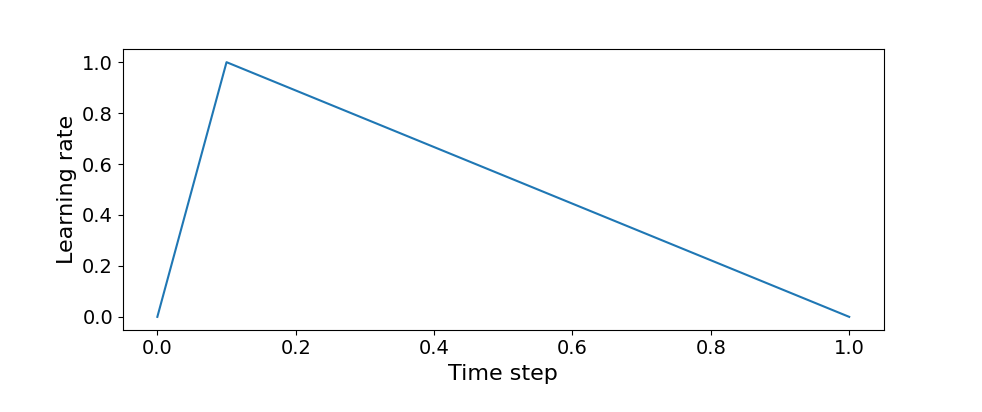
\includegraphics[width=\columnwidth]{figures/warmup-schedule.png}
\caption{Linear warmup learning rate schedule}
\label{fig:warmup-schedule}
\end{center}
\end{figure}

Both models were trained on a system with a single Nvidia T4 GPU.

\begin{figure}
\begin{center}
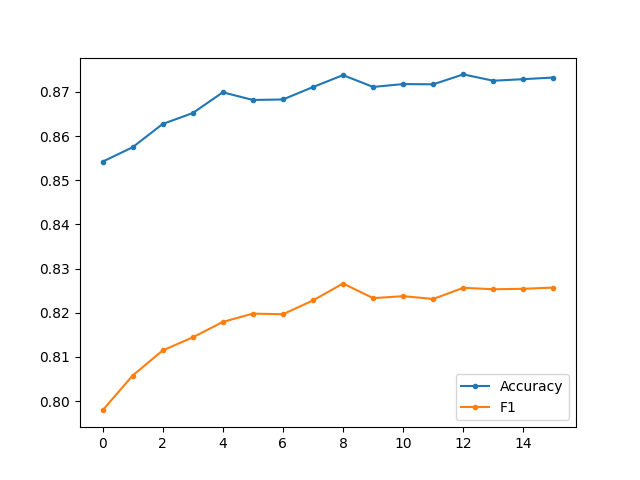
\includegraphics[width=\columnwidth]{figures/train-metrics-distilroberta.png}
\caption{Accuracy and F1 score during training - DistilRoBERTa}
\label{fig:train-metrics-distilroberta}
\end{center}
\end{figure}

\begin{figure}
\begin{center}
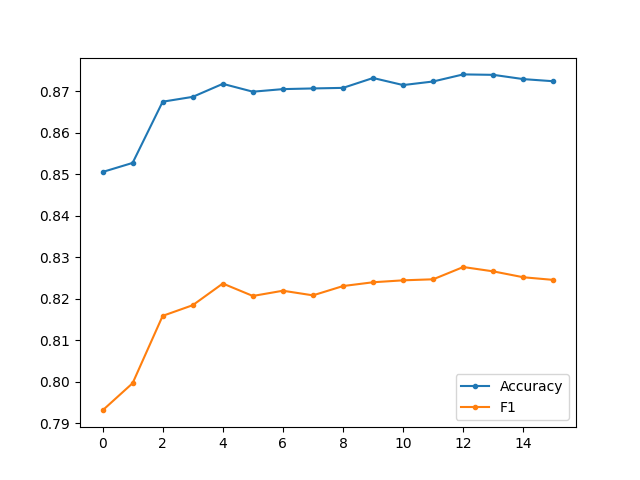
\includegraphics[width=\columnwidth]{figures/train-metrics-roberta.png}
\caption{Accuracy and F1 score during training - RoBERTa}
\label{fig:train-metrics-roberta}
\end{center}
\end{figure}

\subsection{Results} \label{results}

The results are presented in Table~\ref{tab:results}.
All other models significantly outperform the simple cosine similarity baseline using GloVe embeddings.
Expectedly, the SBERT models outperform the Siamese LSTM on accuracy and F1 scores on both the dev and the test.

The accuracy and F1 scores during training are shown for DistilRoBERTa and RoBERTa models in Figure~\ref{fig:train-metrics-distilroberta} and Figure~\ref{fig:train-metrics-roberta}, respectively.

\begin{table*}
\caption{Accuracy and F1 scores on the dev and test sets for the evaluated models.}
\label{tab:results}
\begin{center}
\begin{tabular}{lcccc}
\toprule
 & \multicolumn{2}{c}{Dev set} & \multicolumn{2}{c}{Test set} \\
\midrule
Model & F1 score & Accuracy & F1 score & Accuracy \\
\midrule
Cosine similarity & 36.4 & 37.1 & 35.8 & 36.2 \\
SLSTM & 79.5 & 83.9 & 79.5 & 83.8 \\
RoBERTa & 82.5 & 87.2 & 83.9 & 86.6 \\
DistilRoBERTa & 82.7 & 87.4 & 82.2 & 86.1 \\
\bottomrule
\end{tabular}
\end{center}
\end{table*}

\section{Conclusion} \label{conclusion}

The task of identifying duplicate questions is of particular interest to many Q\&A platforms, as it can help enhance the user experience.
The Quora Question Pairs dataset is an important resource in this area of research. Previous best-performing architectures on this task used Siamese LSTM based models.
An example of such an architecture is the Siamese LSTM model, which won the 2017 Quora Question Pairs Kaggle competition.
We investigated the performance of Sentence-BERT models on this task, and compared them to the winning solution.
We find that Sentence-BERT models outperform the Siamese LSTM architecture on the Quora Question Pairs dataset.
This is in line with expectations since newer pretrained Transformer architectures have dominated the field as of late.

\bibliographystyle{tar2023}
\bibliography{tar2023}

\end{document}

